\section{Introduction}

The idea behind Reinforcement Learning is that an agent (an AI) will learn from the environment by interacting with it (through trial and error) and receiving rewards (negative or positive) as feedback for performing actions.

Formal definition:
\begin{definition}
    Reinforcement learning is a framework for solving control tasks (also called decision problems) by building agents that learn from the environment by interacting with it through trial and error and receiving rewards (positive or negative) as unique feedback.
\end{definition}

\subsection{Framework}

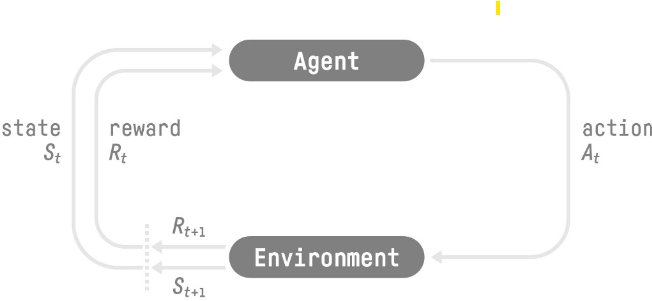
\includegraphics{images/RL_framwork.png}
\begin{enumerate}
    \item Our Agent receives state $S_0$ from the environment.
    \item Based on that state, the agent selects an action $A_0$.
    \item The environment transitions to a new state $S_1$ and provides a reward $R_1$.
\end{enumerate}
This RL loop outputs a sequence of state-action-reward tuples: $(S_0, A_0, R_1, S_1)$. The agent's goal is to maximize the total reward it receives over time.

\subsubsection{Reward Hypothesis}
\begin{definition}
    The reward hypothesis states that all goals can be described by the maximization of the expected cumulative reward.
\end{definition}

\subsection{Markov Property}
RL process might be called \textbf{Markov Decision Process (MDP)} if it satisfies the Markov property. The Markov property states that the future state depends only on the current state and action, not on the past states and actions.

\begin{definition}
    Observations/States are the \textbf{information our agent gets from the environment}.
\end{definition}

It will be good that we are always given a complete description of the state of the world. However, in practice, we might not have access to the complete state of the world. In such cases, we can use the \textbf{observation (partial description of the state)} to represent the state of the world.

\subsubsection{Action Space}

\begin{definition}
    The action space is the set of all possible actions that the agent can take.
\end{definition}
\begin{itemize}
    \item Discrete action space: The agent can take a finite number of actions.
    \item Continuous action space: The agent can take an infinite number of actions.
\end{itemize}

\subsubsection{Reward and the discounting}

The reward is the only feedback to the agent to evaluate its actions. 

The cumulative reward is the sum of all rewards the agent receives over time. \begin{equation}
    R(\tau) = \sum_{t=0}^{\infty} \gamma^t r_t
\end{equation}
where $\tau$ is the trajectory, $r_t$ is the reward at time $t$, and $\gamma$ is the discount factor.

\begin{definition}
    The discount factor $\gamma$ is a value between 0 and 1 that determines the importance of future rewards.
\end{definition}
We have it since the reward in the future is less valuable than the reward now. Typically, $\gamma \in (0.95, 0.99)$.

\subsection{Types of tasks}
\begin{definition}
    A task is an instance of a Reinforcement Learning problem.
    \begin{itemize}
        \item \textbf{Episodic tasks}: Tasks that have a well-defined starting and ending point.
        \item \textbf{Continuing tasks}: Tasks that continue indefinitely.
    \end{itemize}
\end{definition}

\subsubsection{Episodic tasks}
An episodic task creates an episode, which is a sequence of states, actions, and rewards that ends in a terminal state. 

For instance, think about Super Mario Bros: an episode begins at the launch of a new Mario Level and ends when you’re killed or you reached the end of the level.

\subsubsection{Continuing tasks}
Continuing tasks continue indefinitely. In this case, the agent must learn how to choose the best actions and simultaneously interact with the environment.

For example, think about a robot that needs to learn how to walk. The robot will keep walking until the battery runs out.

\subsection{Exploration and Exploitation}

\begin{definition}
    Exploration is the process of trying out new actions to discover the best possible actions.
\end{definition}

\begin{definition}
    Exploitation is the process of selecting the best-known actions to maximize the reward.
\end{definition}

The general trap is that if we exploit too much, we might miss out on better actions. On the other hand, if we explore too much, we might not get enough reward.









